\documentclass{standalone}

\usepackage{tikz}
\usepackage{tkz-euclide}
\usetikzlibrary{calc}
\usetikzlibrary{positioning}
\usetikzlibrary{arrows.meta}

\usepackage{times}


\begin{document}
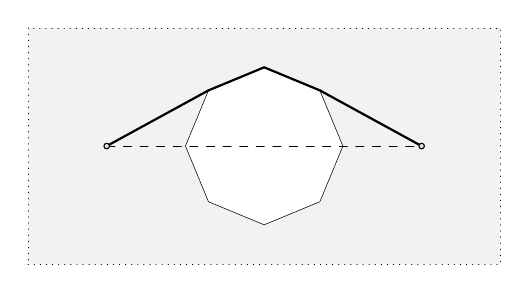
\begin{tikzpicture}[%
  >={Stealth[scale=1.0]},
  scale=1.0,
  % yscale=0.8,
]

  \tkzDefPoint(-3.0, -1.5){A}
  \tkzDefPoint(3.0, -1.5){B}
  \tkzDefPoint(3.0, 1.5){C}
  \tkzDefPoint(-3.0, 1.5){D}

  \tkzDrawPolygon[dotted,color=black,fill=black!5](A,B,C,D)

  \tkzDefPoint(0.0, 0.0){M}
  \tkzDefPointOnCircle[R = center M angle 0 radius 1]\tkzGetPoint{B1}
  \tkzDefPointOnCircle[R = center M angle 45 radius 1]\tkzGetPoint{B2}
  \tkzDefPointOnCircle[R = center M angle 90 radius 1]\tkzGetPoint{B3}
  \tkzDefPointOnCircle[R = center M angle 135 radius 1]\tkzGetPoint{B4}
  \tkzDefPointOnCircle[R = center M angle 180 radius 1]\tkzGetPoint{B5}
  \tkzDefPointOnCircle[R = center M angle 225 radius 1]\tkzGetPoint{B6}
  \tkzDefPointOnCircle[R = center M angle 270 radius 1]\tkzGetPoint{B7}
  \tkzDefPointOnCircle[R = center M angle 315 radius 1]\tkzGetPoint{B8}
  \tkzDrawPolygon[draw=black,fill=white](B1,B2,B3,B4,B5,B6,B7,B8)

  \tkzDefPoint(-2.0, 0.0){p}
  \tkzDefPoint(2.0, 0.0){q}

  \tkzDrawSegments[thick](p,B4 B4,B3 B3,B2 B2,q)

  \tkzDrawSegment[dashed](p,q)
  \tkzDrawPoints(p,q)

\end{tikzpicture}
\end{document}
